\documentclass[a4paper,12pt]{article}
\usepackage[utf8]{inputenc}
\usepackage[margin=1in]{geometry}
\usepackage{amsmath}
\usepackage{amsthm}
\usepackage{alltt}
\setlength{\parindent}{0pt}
\setlength{\parskip}{5pt}
\usepackage{newcent}
\selectfont
\theoremstyle{definition}
\newtheorem{exmp}{Exemple}[section]
\renewcommand*\contentsname{Sommaire}
\usepackage{color}
\usepackage{scrextend}
\usepackage{multicol}
\setlength{\emergencystretch}{2pt}

\title{ {\bf Rapport du Projet }\\
        (environ 30 pages à faire) }
\author{ Yann  Kergutuil \quad
         Rolih Meynard   \quad
         John  Gliksberg \quad \\
         M1 MIHPS @ UVSQ }
\date{}

\begin{document}
\maketitle

\tableofcontents

\pagebreak

Le principal objectif du projet est de mettre en valeur
des champs lexicaux dans un ensemble de corpus de texte.
En effet, le travail à effectuer consiste à extraire des
catégories de mots, à savoir des champs lexicaux à travers
de nombreux documents.
Les documents auquels on se réfère sont exclusivement des
articles de Wikipédia.

Les démarches envisagées sont, pour l'essentiel, basées sur
l'utilisation de matrices ayant différents paramètres.
Les paramètres sont entre autres des mots, des distances et
aussi des occurences. D'autres méthodes sont appliquées,
notamment sur le calcul de distances et de matching par rapport
à des dictionnaires de mots.

Le sujet de ce projet traite de l'analyse statistique
et des méthodes de clustering.

\section{État de l'art}

\subsection{L'extraction d'information}

Le coeur du projet repose sur la récupération d'information
({\it information retrieval}).
Une des principales applications de cette méthode
que l'on peut citer est la recherche de résumés
d'articles scientifiques dans les bases de données.
Ainsi, dans le cadre de la recherche médicale il peut être
question de trouver l'ensemble des résumés d'articles dans une
base de données qui traite d'un sydrôme particulier.
Pour obtenir ces articles, la solution consistera à faire une requête
à partir de mots clés qui sont pertinents au syndrôme.
Ensuite, le système de récupération devra, d'une part,
comparer la requête aux différents documents dans la base de données
et, d'autre part, présenter à l'utilisateur les documents qui sont
à la fois pertinents et rangés dans un ordre suivant
le volume d'information contenu dans l'article.

Deux exemples concrets pour illustrer la récupération d'information :

\paragraph{Exemple 1.1}
Requête pour la recherche dans une catégorie de résumés
d'articles médicaux: {\it les symptômes d'une grippe}

Ainsi, tous les articles dont le contenu est lié aux symptômes
%de la grippe seront répertoriés par le système.

\paragraph{Exemple 1.2}
Requête sur la recherche d'articles universitaires

Les revues sont un autre exemple d'applications
de récupération d'information.

Ainsi, si nous lançons la requête suivante nous avons:

\begin{table}[!htb]
\begin{center}
\begin{tabular}{l p{6cm}}
\bf Mots clés & \bf Resultats \\
Computer science engineering  & \it Nothing found \\
Computing science engineering
& IEEE: Computing in Science and Engineering
\end{tabular}
\caption{Recherche d'articles universitaires}
\end{center}
\end{table}

Le système de récupération d'information est censé être
insensible à la moindre erreur ou le moindre changement
de lettre dans la requête.
Dans l'exemple 1.2, nous pouvons remarquer que la revue IEEE
répond à la seconde requête.
De cet exemple, nous pouvons inférer que dans beaucoup de cas
la comparaison de mots peut générer des résultats inattendus.

Par ailleurs, un domaine bien connu dans la récupération
d'information concerne les moteurs de recherche Web.
Dans ce genre de systèmes, les requêtes sont très courtes,
et de nombreux documents trouvés peuvent être des informations
qui sortent du cadre du sujet attendu par l'utilisateur.
Ainsi, le classemment du resultat de la recherche est un
critère d'efficacité du moteur de recherche.

\subsection{Prétraitement des documents et des requêtes}

Dans cette partie, il s'agit d'étudier le prétraitement qui
est mis en oeuvre au préalable.
Au niveau de la récupération d'information,
les mots clés qui résument l'information à propos du thème
d'un document sont appelés termes.
De ce fait, une étape essentielle dans la mise en valeur
de champs lexicaux est de créer une liste de tous les termes
dans un recueil de documents, ainsi appelé index.
Pour chaque terme, une liste de tous les documents contenant
ce terme particulier est stockée.

\subsubsection{Indexation inversée}

La principale structure donnée au sein d'un système
de recupération d'information s'agit de l'indexation
inversée. De façon usuelle, un index inversée établit
une relation entre les termes et leurs occurences dans un
document donné. Nous pouvons ainsi illustrer un exemple
d'index inversée:

\paragraph{Exemple 2.1}
Un exemple d'index inversée qui représente les termes
avec leurs occurences.

\begin{table}[h]
\begin{center}
\begin{tabular}{l l}
\bf Terme & \bf Liste d'occurences \\
programme & 2301, 1268, ..., 74896, 47123, 741 \\
matrice   & 4789, 4987, 1236, 7869, ..., 4682, 6321, 1978 \\
parallèle & 4781, 1247, 963, 4707, ..., 4136, 1247, 7841
\end{tabular}
\caption{Dictionnaire}
\end{center}
\end{table}

Dans l'exemple précédent, le dictionnaire fournit une courte
liste des termes présents dans les documents, et aussi une
liste correspondante aux placements de ces termes. Nous pouvons
constater que l'index inversé présenté ne donne pas les
identifiants des documents contenant des termes.
{\color{red} On appelle ce type d'index un index de
schéma-indépendant compte-tenu qu'aucune hypothèse
n'est faite à propos du choix de stockage des documents}.

Un index inversé peut être défini à partir de 4 méthodes:

\begin{addmargin}{.5cm}

\begin{tabular}{l p{11cm}}
\tt .premier(t) & retourne la première position à
                  laquelle le terme t apparait dans
                  l'ensemble du document
\end{tabular}

\begin{tabular}{l p{11cm}}
\tt .dernier(t) & retourne la dernière position à
                  laquelle le terme t apparait dans
                  l'ensemble du document
\end{tabular}

\begin{tabular}{l p{8.2cm}}
\tt .prochain(t, actuelle) & retourne la première position
                             occurence du terme t après la
                             position actuelle
\end{tabular}

\begin{tabular}{l p{8.1cm}}
\tt .precedent(t, actuelle) &
\end{tabular}

\end{addmargin}

Ce procédé est appelé un {\it inverted index},
littéralement index inversé.

Avant d'effectuer un index, deux étapes de prétraitements
doivent être réalisées, à savoir l'élimination de tous
les mots non pertinents et l'affichage du radical.

L'élimination de mots a pour principe de supprimer les mots
qui n'apportent pas d'information sur ce document.
On peut s'attendre à les trouver dans la majorité des documents
\---- en particulier, on peut s'attendre à ce qu'ils ne soient
pas plus fréquents dans le document considéré que dans le corpus
global de documents.

On peut rechercher ces types de mots en analysant en effet
leur fréquence, ou exclure, sans analyse, des mots qu'on prévoit
comme négligeables (par exemple les articles définis et indéfinis,
les mots de liaison ({\it car}, {\it avant}, {\it aussi}, etc...)).
Dans notre cahier des charges on doit avoir aussi peu d'à priori
que possible sur le texte à analyser donc on se contente d'exclure
les mots trop courts ({\it i.e.} moins de trois caractères)
et on pourrait/devrait analyser les matrices de fréquences pour
déterminer les mots sans information.

L'affichage du radical est la procédure qui vise à réduire
chaque mot qui est conjugué ou qui a son propre suffixe.
Par exemple,

\begin{center}
\begin{tabular}{l}
{\bf program}mation \\
{\bf program}mable  \\
{\bf program}mer    \\
{\bf program}me     \\
\end{tabular}
\end{center}

Dans le cadre de notre projet, on n'a pas effectué
de détermination du radical car on traite des types
de mots variés dans de nombreuses langues,
ainsi les règles de construction sont trop complexes.
De plus, comme c'est souvent le cas, cela pousserait
dans de nombreux cas à réunir comme de la même famille
des mots très différents. Par exemple,

\begin{center}
\begin{multicols}{3}
to present \\
he presents \\
a presentation \\
elle se présente \\
\columnbreak
the present \\
presents \\
offre un présent \\
\columnbreak
il est présent \\
live the present \\
à présent
\end{multicols}
\end{center}

\subsection{Le modèle espace vertoriel}

Le modèle espace vectoriel développe commme principale idée
de créer une matrice de mot-document ({\tt matrix\_words})
dans laquelle chacun des documents est représenté par
un vecteur colonne {\color{red} (c'est pas matrix\_docs ça?)}.
Le vecteur a des valeurs non-nulles dans les positions qui font
référence aux termes qui peuvent être présents dans les documents.
Ainsi, concrètement chaque ligne détient un terme et les entrées
sont nulles pour les positions correspondant aux documents
contenant le terme.
Chaque terme a un numéro identifiant.
L'exemple ci-dessous représente une matrice de mot-document:

\begin{center}
\begin{tabular}{ccc}
Document 1 & Document 2 & Document 3 \\
1          & 2          & 3 \\
4          & 5          & 6 \\
7          & 8          & 9
\end{tabular}
\end{center}

Identifiants des mots:

\begin{center}
\begin{tabular}{ll|ll}
calcul        & = 1 & bug         & = 6 \\
programmer    & = 2 & scalabilité & = 7 \\
code          & = 3 & matrice     & = 8 \\
développement & = 4 & vecteur     & = 9 \\
test          & = 5
\end{tabular}
\end{center}

Une fois la matrice de mot-document créée,
il convient de calculer l'occurrence des termes
dans les documents.

La matrice de mot-document que l'on a construit est pleine.

\subsubsection{Requête de matching et modélisation de performance}

La  requête de matching consiste de trouver les documents qui sont
pertinents à une requête $q$ particulière.
De manière générale, ce type de requête est réalisé à partir
de la mesure distance cosinus.
Par conséquent, un document $D(j)$ est considéré pertinent
si l'angle entre la requête $q$ et $D(j)$ est assez minime.
Ainsi $D(j)$ est extrait si l'on a

\[
	cos \left[ \theta(q, D(j)) \right]
	= \frac{q^T \times D(j)}
	       {\left|\left| q    \right|\right| _2 \times
	        \left|\left| D(j) \right|\right| _2} > tol
\]

$tol$ est un seuil de tolérance prédéfini.
Si la tolérance est réduite,
les documents ont davantage retournés,
ce qui signifie qu'ils sont pertinents à la requête.
Cependant, le risque est qu'avec une tolérance réduite,
des documents non pertinents peuvent être aussi retournés.

Dans l'extraction d'information,
il est possible de mesurer la performance de la modélisation:

\[
	\mbox{Précision :} \quad P = \frac{D(r)}{D(t)}
\]

$D(r)$ représente le nombre de documents pertinents extraits
et $D(t)$ représente le nombre total de documents extraits.

\subsection{Indexation sémantique latente}

{\bf Définitions}

L'analyse sémantique latente est une technique sur le traitement
des langues naturelles et qui se repose sur la sémantique vectorielle.

L'indexation sémantique latente est un procédé qui effectue une relation
entre un goupe de documents et les termes contenus dans ces documents.

{\bf Matrice des occurences}

Dans le cadre de l'indexation sémantique latente,
on est amené à construire une matrice des occurences.
Cette matrice contient l'occurence des termes dans les documents.
Il s'agit d'une matrice creuse.

Tous les ``termes'', venant de l'ensemble du corpus de texte,
de la matrice sont des mots qui sont tronqués à leur radical.


\pagebreak
\section{Conception séquentielle}

\subsection{Vue d'ensemble}

\paragraph{Problème donné}

On part, dans notre projet, d'un gros fichier
``type wikipedia'' qui représente un corpus de documents.
\begin{addmargin}{.5cm}
\begin{verbatim}
[[Document 1]]
Texte, texte
[[File:filename.ext|arg]]
Texte, texte

[[Document 2]]
Plus de texte
\end{verbatim}
\end{addmargin}

\paragraph{But}

On veut déterminer les champs lexicaux de ce corpus de document.

Par ceci on veut dire déterminer des groupes de mots
qui ont une utilisation (à défaut d'un sens, qu'on ne
peut pas déterminer automatiquement) similaire.
De même on veut pouvoir montrer comment des documents
sont liés ensemble.

On réduit le problème en sous-problèmes \----
tout d'abord on prépare les documents
(découpage du fichier wiki en documents individuels,
conversion en ASCII 1 octet = 1 charactère),
puis on crée une liste des mots avec occurences
d'un document, qu'on intègre à un dictionnaire
existant, puis

\paragraph{Conditions}

On veut faire aussi peu de suppositions sur les
documents et les mots que possible.

En effet on s'autorise certaines règles basiques pour
reconnaître un mot et des méthodes statistiques pour
faire ressortir les mots importants par leur usage
mais jamais par des listes prédéfinies.
Si besoin, et dans le meilleur des cas, on peut construire
des listes à partir des analyses, comme par apprentissage.


\pagebreak
\section{Maison de la Simulation}



\pagebreak
\section{Parallélisation}

Notre code est intrinsèquement divisé en deux étape,
la première étant l'initialisation du dictionnaire,
la seconde est le calcul matriciel qui permet de
converger vers un résultat.

L'initialisation est la partie qui prend le moins
de temps à l'exécution,
phénomène d'autant plus remarquable si la taille des
documents et leur nombre augmente.
Nous avons de plus remarqué qu'il était compliqué de répartir
cette initialisation sur plusieurs noeuds MPI sans
engendrer une graphe de communication très chargé.
En effet les identifiants associés à un document
ou à un mot sont créés si ce mot/documents est relevé
pour la première fois dans l'initialisation.
Par exemple on aura alors le cas où deux noeuds
découvrent à des instants différents dans leur processus
de création de dictionnaire un document.
Ce dit-document aura donc un identifiant i sur
le premier noeud et un identifiant j dans le second
or nous devons avoir un identifiant unique pour
un élément du dictionnaire.

Nous nous sommes donc concentrés sur la parallélisation
du calcul matriciel.
Une fois le dictionnaire et son indexation inversée
établis nous savons que les matrices de fréquence qui les
représentent ne seront plus modifiées au cours de l'algorithme.
Ainsi nous avons décidé de distribuer à chacun des sites
ces deux matrices ({\it Docs} et {\it Words}).
Notre algorithme consiste à chaque étape à comparer
les documents/mots deux à deux.
Afin que la charge de travail entre processus MPI soit
équilibrée chaque processus devra effectuer

\[ \frac{N_d \times (N_d+1)}{P \times 2}
 + \frac{N_w \times (N_w+1)}{P \times 2} \]

comparaisons à chaque étape
(avec $N_d$ le nombre total de documents, $N_w$ le nombre total de mots et $P$ le nombre de processus).

\begin{figure}[h]
\begin{center}
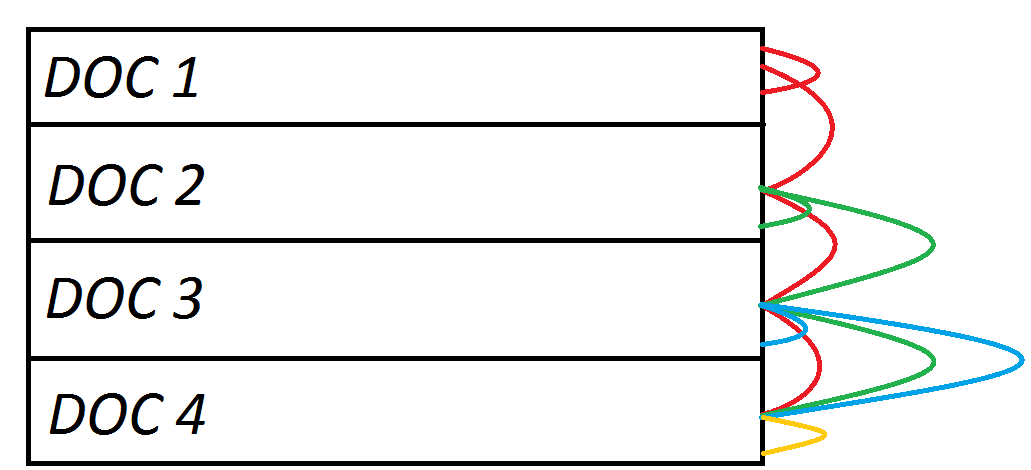
\includegraphics[height=1.5in]{cr/1}
\caption{Opérations inter-documents}
\end{center}
\end{figure}

Pour être plus précis: \newline

le processus 1 compare le document 1 avec les documents 1,2,3 et 4\newline
le processus 2 compare le document 2 avec les documents 2,3 et 4\newline
le processus 3 compare le document 2 avec les documents 3 et 4\newline
le processus 4 compare le document 2 avec les documents 4.

\newpage 
Nous obtenons donc le graphe suivant: 
 
\begin{figure}[h]
\begin{center}
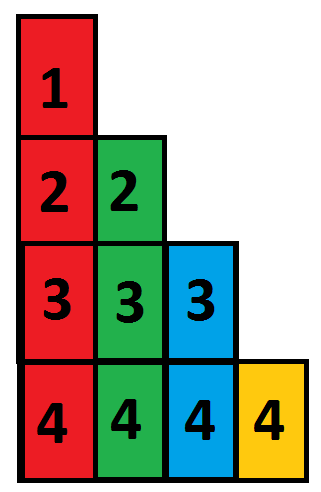
\includegraphics[height=1.5in]{cr/2}
\caption{Charge déséquilibré}
\end{center}
\end{figure}

On remarque que dans notre exemple ci-dessus, si nous souhaitons le répartir sur quatres processus MPI de façon naïf, la charge 
de travail ne sera pas  équilibré (rapport de 4 entre le processus 1 et le dernier). Il convient de répartir plus intéligement commes dans l'exemple suivant où 
il y a 10 documents, cela représente 55 combinaisons possible de comparaison. Ainsi nos 5 processus devront traiter exactement 11 combinaisons.

\begin{figure}[h]
\begin{center}
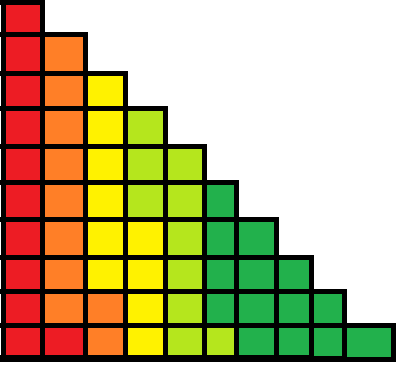
\includegraphics[height=1.5in]{cr/4}
\caption{Charge équilibré}
\end{center}
\end{figure}


Une étape est constitué des deux appels de fonctions suivant :

\begin{verbatim}
Matrix_Docs  = dist_polia(Docs, Matrix_Words)
Matrix_Words = dist_polia(Words, Matrix_Docs)
\end{verbatim}

Ici la fonction calcul une nouvealle matrice de distance à partir du matrice de fréquence et la matrice de distance complémentaire.
Les processus savent donc sur quelle plage de donnée
ils effectuent leurs calculs.
Une étape consiste à recalculer les matrices de distances
{\tt Matrix\_Docs} et {\tt Matrix\_Words}.
Ainsi entre deux appels de la fonction {\tt dist\_polia}
chaque processus doit recevoir les nouvelles distances que
les processus restant viennent de calculer.


\end{document}
